\chapter{Why Do We Need Calculus}
\label{sec:course intro}
%\pagenumbering{arabic}

\epigraph{\textbf{Calculus}: A branch of mathematics using the idea of a limit and generally divided into two parts: integral and differential calculus. }{\textit{Penguin Dictionary of Mathematics}}


\section{Course Overview}
\label{sec:overview}
These lecture notes cover the same material as the lectures for \textbf{MAT1001 Differential Calculus}. They will be updated during the module so please check back regularly for the latest version, the date of the most recent update is shown on the front page. In particular, most of the figures used in the lectures are hand drawn and it takes some time to produce good quality digital versions of these.\\

It is important to note that \textbf{reading these notes is not a substitute for attending the lectures and tutorials!} While I have included everything that I intend to cover in the lectures, and have often given more detail in these notes, the direction that we go in lectures will be guided by student questions and the example problems that you are given to solve. These are not reflected in the notes as I cannot anticipate all of the questions that may be asked. If you want to pass the module then the best way to do this is to attend the lectures and tutorials and to solve all of the practice problems that you are given.\\

In week one there was  overview information about the module including a rough schedule, how you will be assessed, and how to contact me. That will not be duplicated here and can be found on the module's virtual learning environment (VLE) page. If you need have any questions during the module then you can send me an \href{mailto:rossc@edgehill.ac.uk}{email} or come by my office during the office hour times. The module reading list, available on the VLE, contains details of recommended and supplementary reading for the module, there will frequently be suggested reading given to complement the material from a given weeks lecture. In these notes I will occasionally cite one of these books in the lecture notes, there will also be extra information and resources given in \cref{sec:further reading}. My favourite reference for much of this material is \citep{riley_mathematical_2006}, which covers all the areas of mathematics that we need for this course.\\

We will mainly be using content from chapters 1, 2, and parts of 27 from \citep{riley_mathematical_2006}.  Another good resource is the calculus page on the website \href{https://tutorial.math.lamar.edu/classes/calci/calci.aspx}{Paul's Online Notes}. There are lots of examples given there, some of which I have included in this lecture notes.\\

Another book that I have sometimes used is \citep{jordan2008mathematical}, it contains lots of background material but does not always have the simplest explanations. For numerical methods \citep{lissamen2004mei} contains a lot of material, and there are several copies in the library.\\


\section{Why Calculus}
\label{sec:why calculus}
\epigraph{\textbf{So what does calculus add for me?} It provides a way for us to construct relatively simple quantitative models of change, and to deduce their consequences. }{\textit{\href{https://math.mit.edu/~djk/calculus_beginners/chapter00/section02.html}{MIT Calculus for Beginners}}}

Calculus is an important topic in mathematics and at its most basic is the study of how functions change. It makes an appearance whenever we are interested in solving an optimisation problem, e.g. finding the best solution to a given problem. This could be finding out the largest area that can be enclosed by a fence of a given length, or what the fastest way to travel between two different points is. One example of this is sometimes called the \textbf{Ocado} or \textbf{vehicle routing problem} and wants to find the optimal route for a delivery van\footnote{More info on this can be found \href{https://www.cardiff.ac.uk/news/view/2585000-improving-vehicle-routing-with-ocado-group}{here}. Sometimes the Ocado problem refers to routing of the robots that pick up groceries in the warehouse which is another example of a vehicle routing problem.}. \\

\begin{figure}[ht]
    \centering
    %\pdftooltip{
    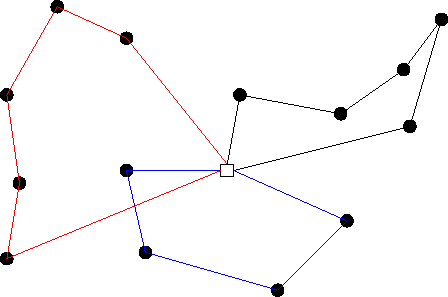
\includegraphics[width=0.35\textwidth, alt ={A schematic of the vehicle routing problem.}]{figures/vehicle_routing_problem}
    %}{. }
    \caption{A schematic of the vehicle routing problem. This is a programming problem where you want to find the optimal set of routes for a fleet of vehicles to travel when making deliveries to a given set of customers, the dots in the figure. This sort of optimisation problem is important for any delivery service as making their routes more efficient can save them money. }
\label{fig: vehicle routing}
\end{figure}

You may be thinking, ``that all sounds sensible in mathematics or physics, but as a computer science why should I care about calculus?'' If so you are not alone, many people ask the same question and there are many answers given online. For example the Medium post \href{https://medium.com/@18bhavyasharma/the-use-of-calculus-in-computer-science-a6917dbe33b9}{The uses of Calculus in Computer Science} highlights several areas:
\begin{itemize}
%\setlength{\itemsep}{-5pt}
    \item \textbf{Algorithms and optimisation:}  As highlighted above, whenever you have an optimisation problem calculus invariably rears its head.
    \item \textbf{Numerical analysis/ Computer graphics and computer vision:} Calculus provides a language for solving complex physical and mathematical problems that we are unable to solve by hand. This is important if you want to simulate a physical system, whether in a piece of scientific research or because you are designing a computer game, but also in graphics rendering and computer vision where you need to understand and simulate the path that light rays will follow.
   \item \textbf{AI and machine learning:} Most machine learning algorithms involve calculus in their optimisation and training.
   \item \textbf{Data science:} Much of data science involves statistical and mathematical modelling to analyse and understand the data. Understanding these techniques relies on understanding calculus. 
\end{itemize}
This all goes to show that calculus is an essential tool in many field beyond pure mathematics and is indispensable for Physicists, Engineers, and computer programmers. \\

\begin{figure}[ht]
    \centering
    %\pdftooltip{
    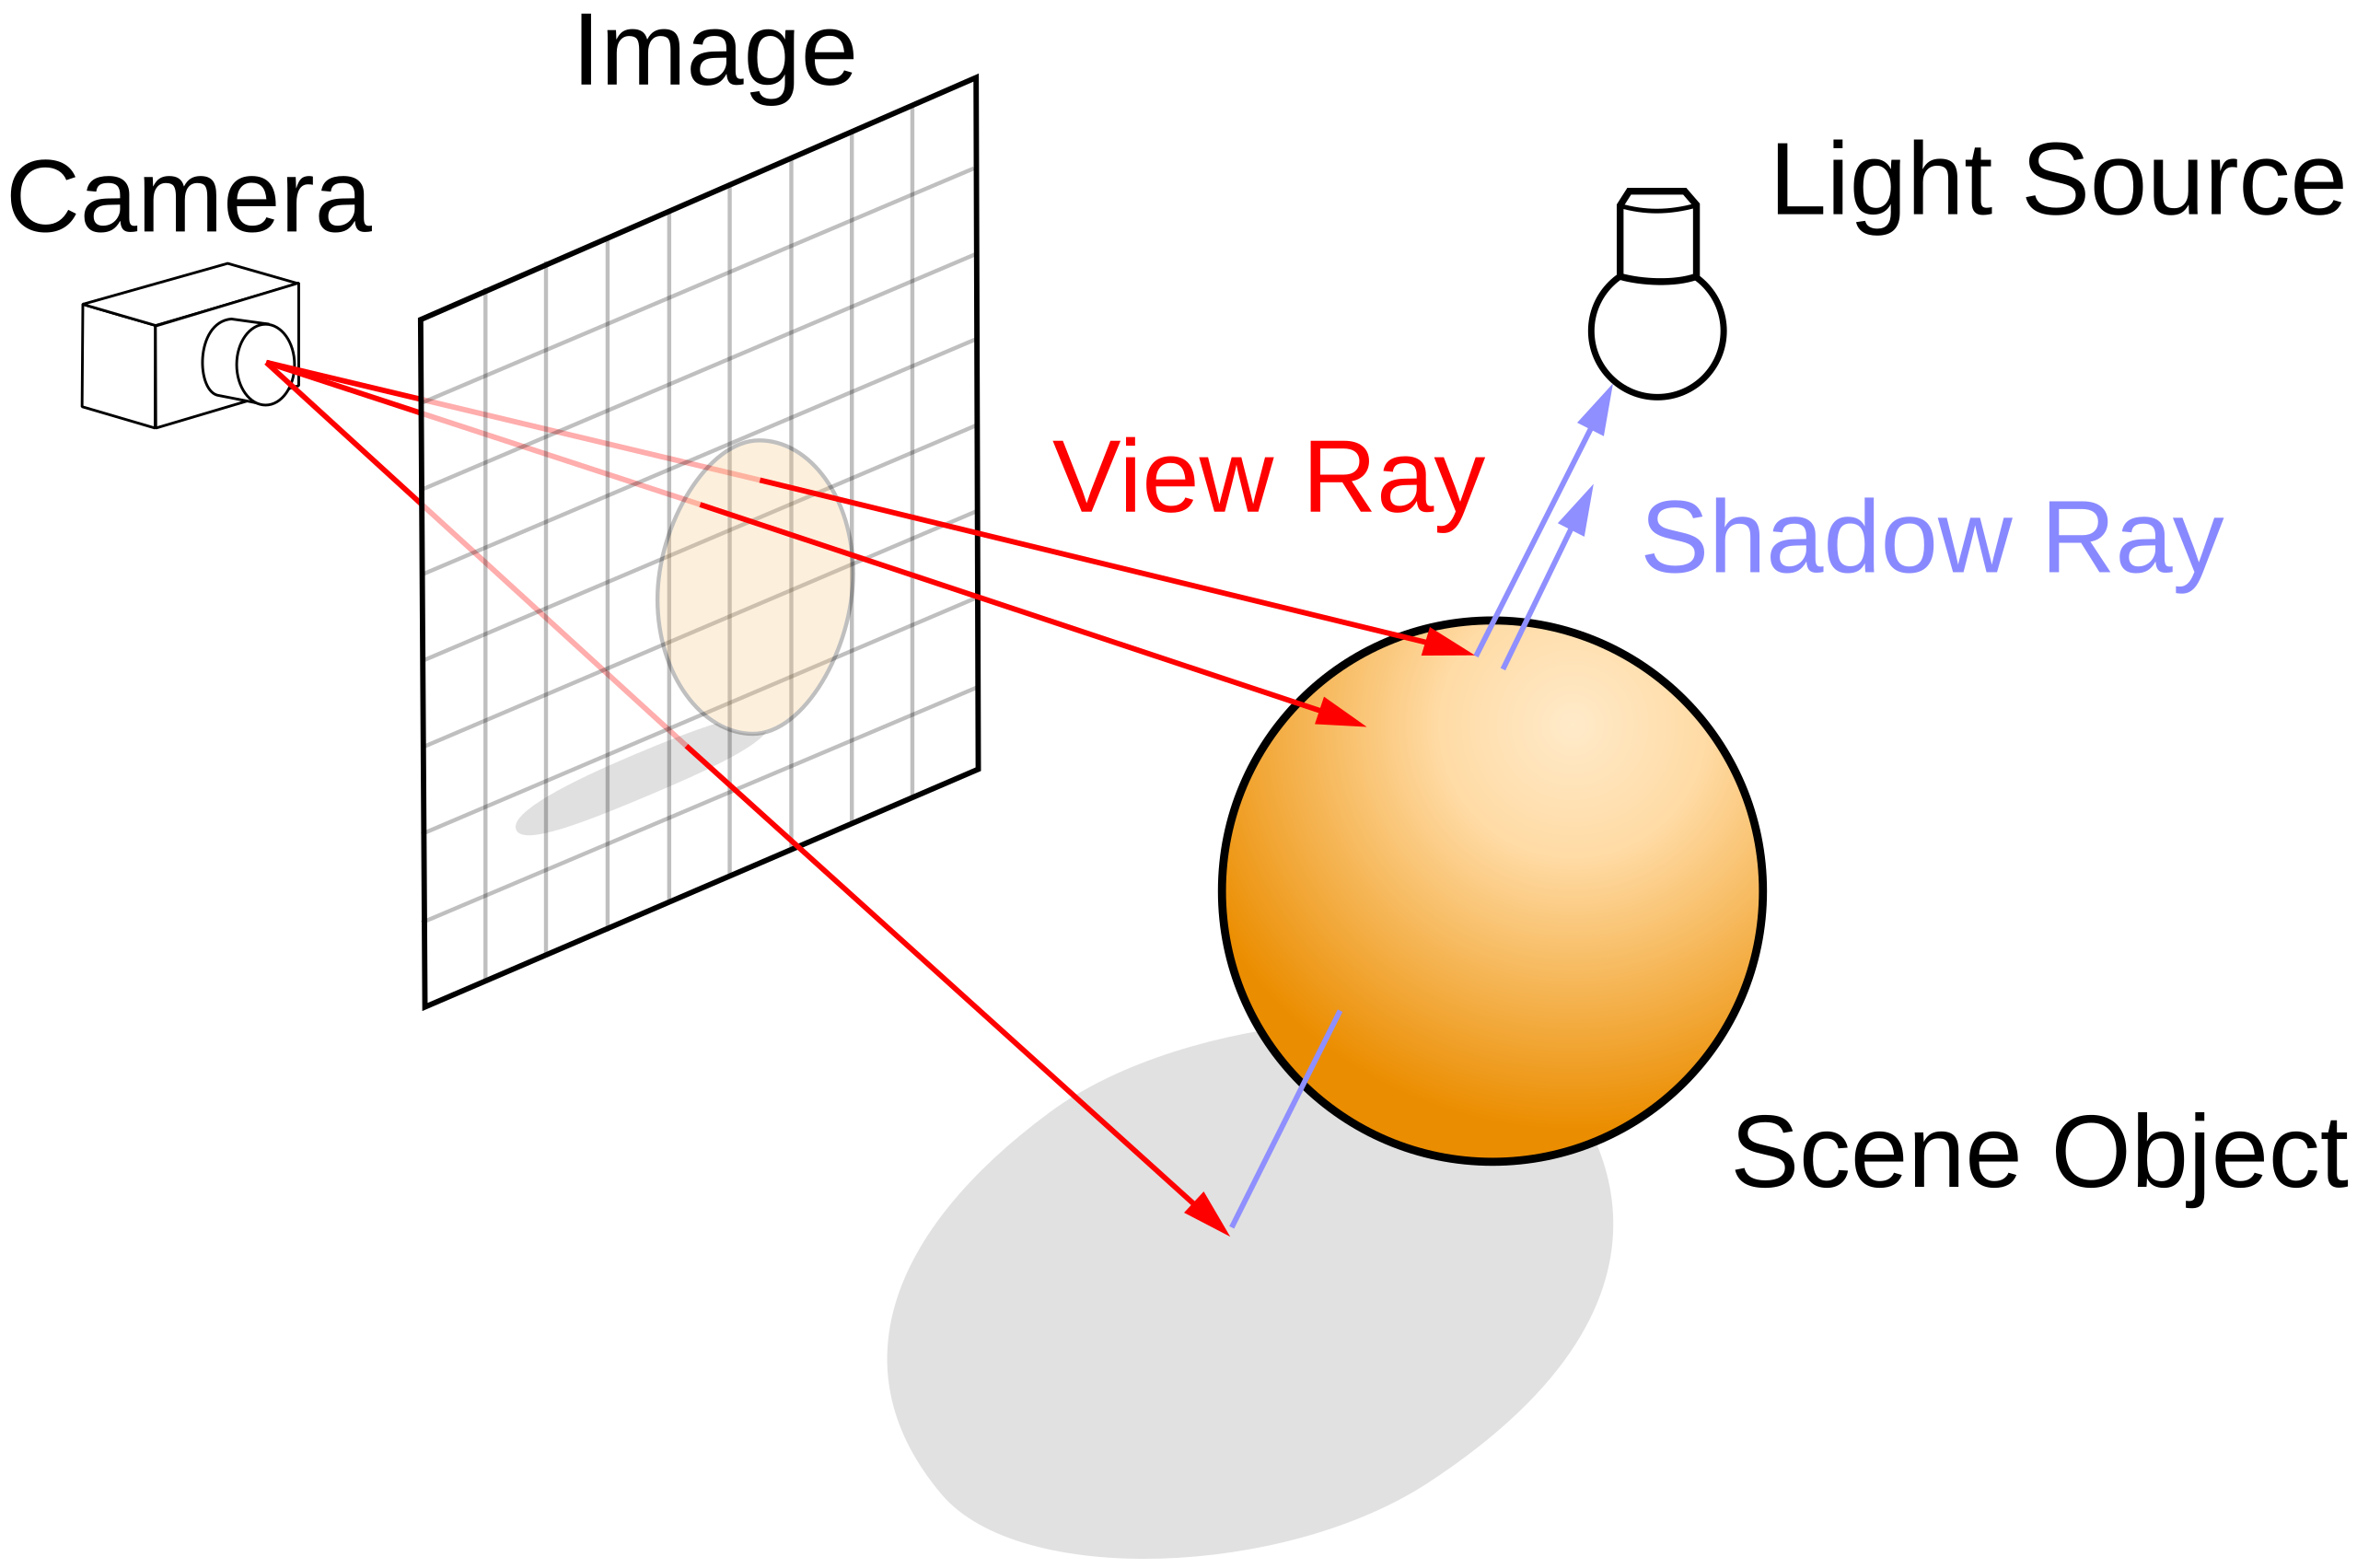
\includegraphics[width=0.6\textwidth, alt = {A schematic of ray tracing.}]{figures/Ray_trace_diagram}
    %}{A schematic of ray tracing. }
    \caption{A schematic showing how a ray tracung algorithm works to build up an image by extending light rays. This image was made by \href{https://commons.wikimedia.org/wiki/File:Ray\_trace\_diagram.svg}{Henrik} for Wikimedia Commons.}
\label{fig: ray tracing}
\end{figure}


Calculus is separated into two main areas: \textbf{\gls{Differentiation}} and \textbf{\gls{Integration}}. Differentiation is the study of how quickly or slowly a function varies. If we have a a graph of a function the derivative is the gradient to this graph, this notion will be made precise in a later section. Integration is the ``opposite'' of differentiation and corresponds to finding the area under the graph of a function.\\

Both concepts can be extended to much more abstract settings but the intuition gained from thinking about graphs of functions, their gradients, and the area under them, will set you in good stead for everything that comes after this.\\

\begin{figure}[ht]
    \centering
    %\pdftooltip{
    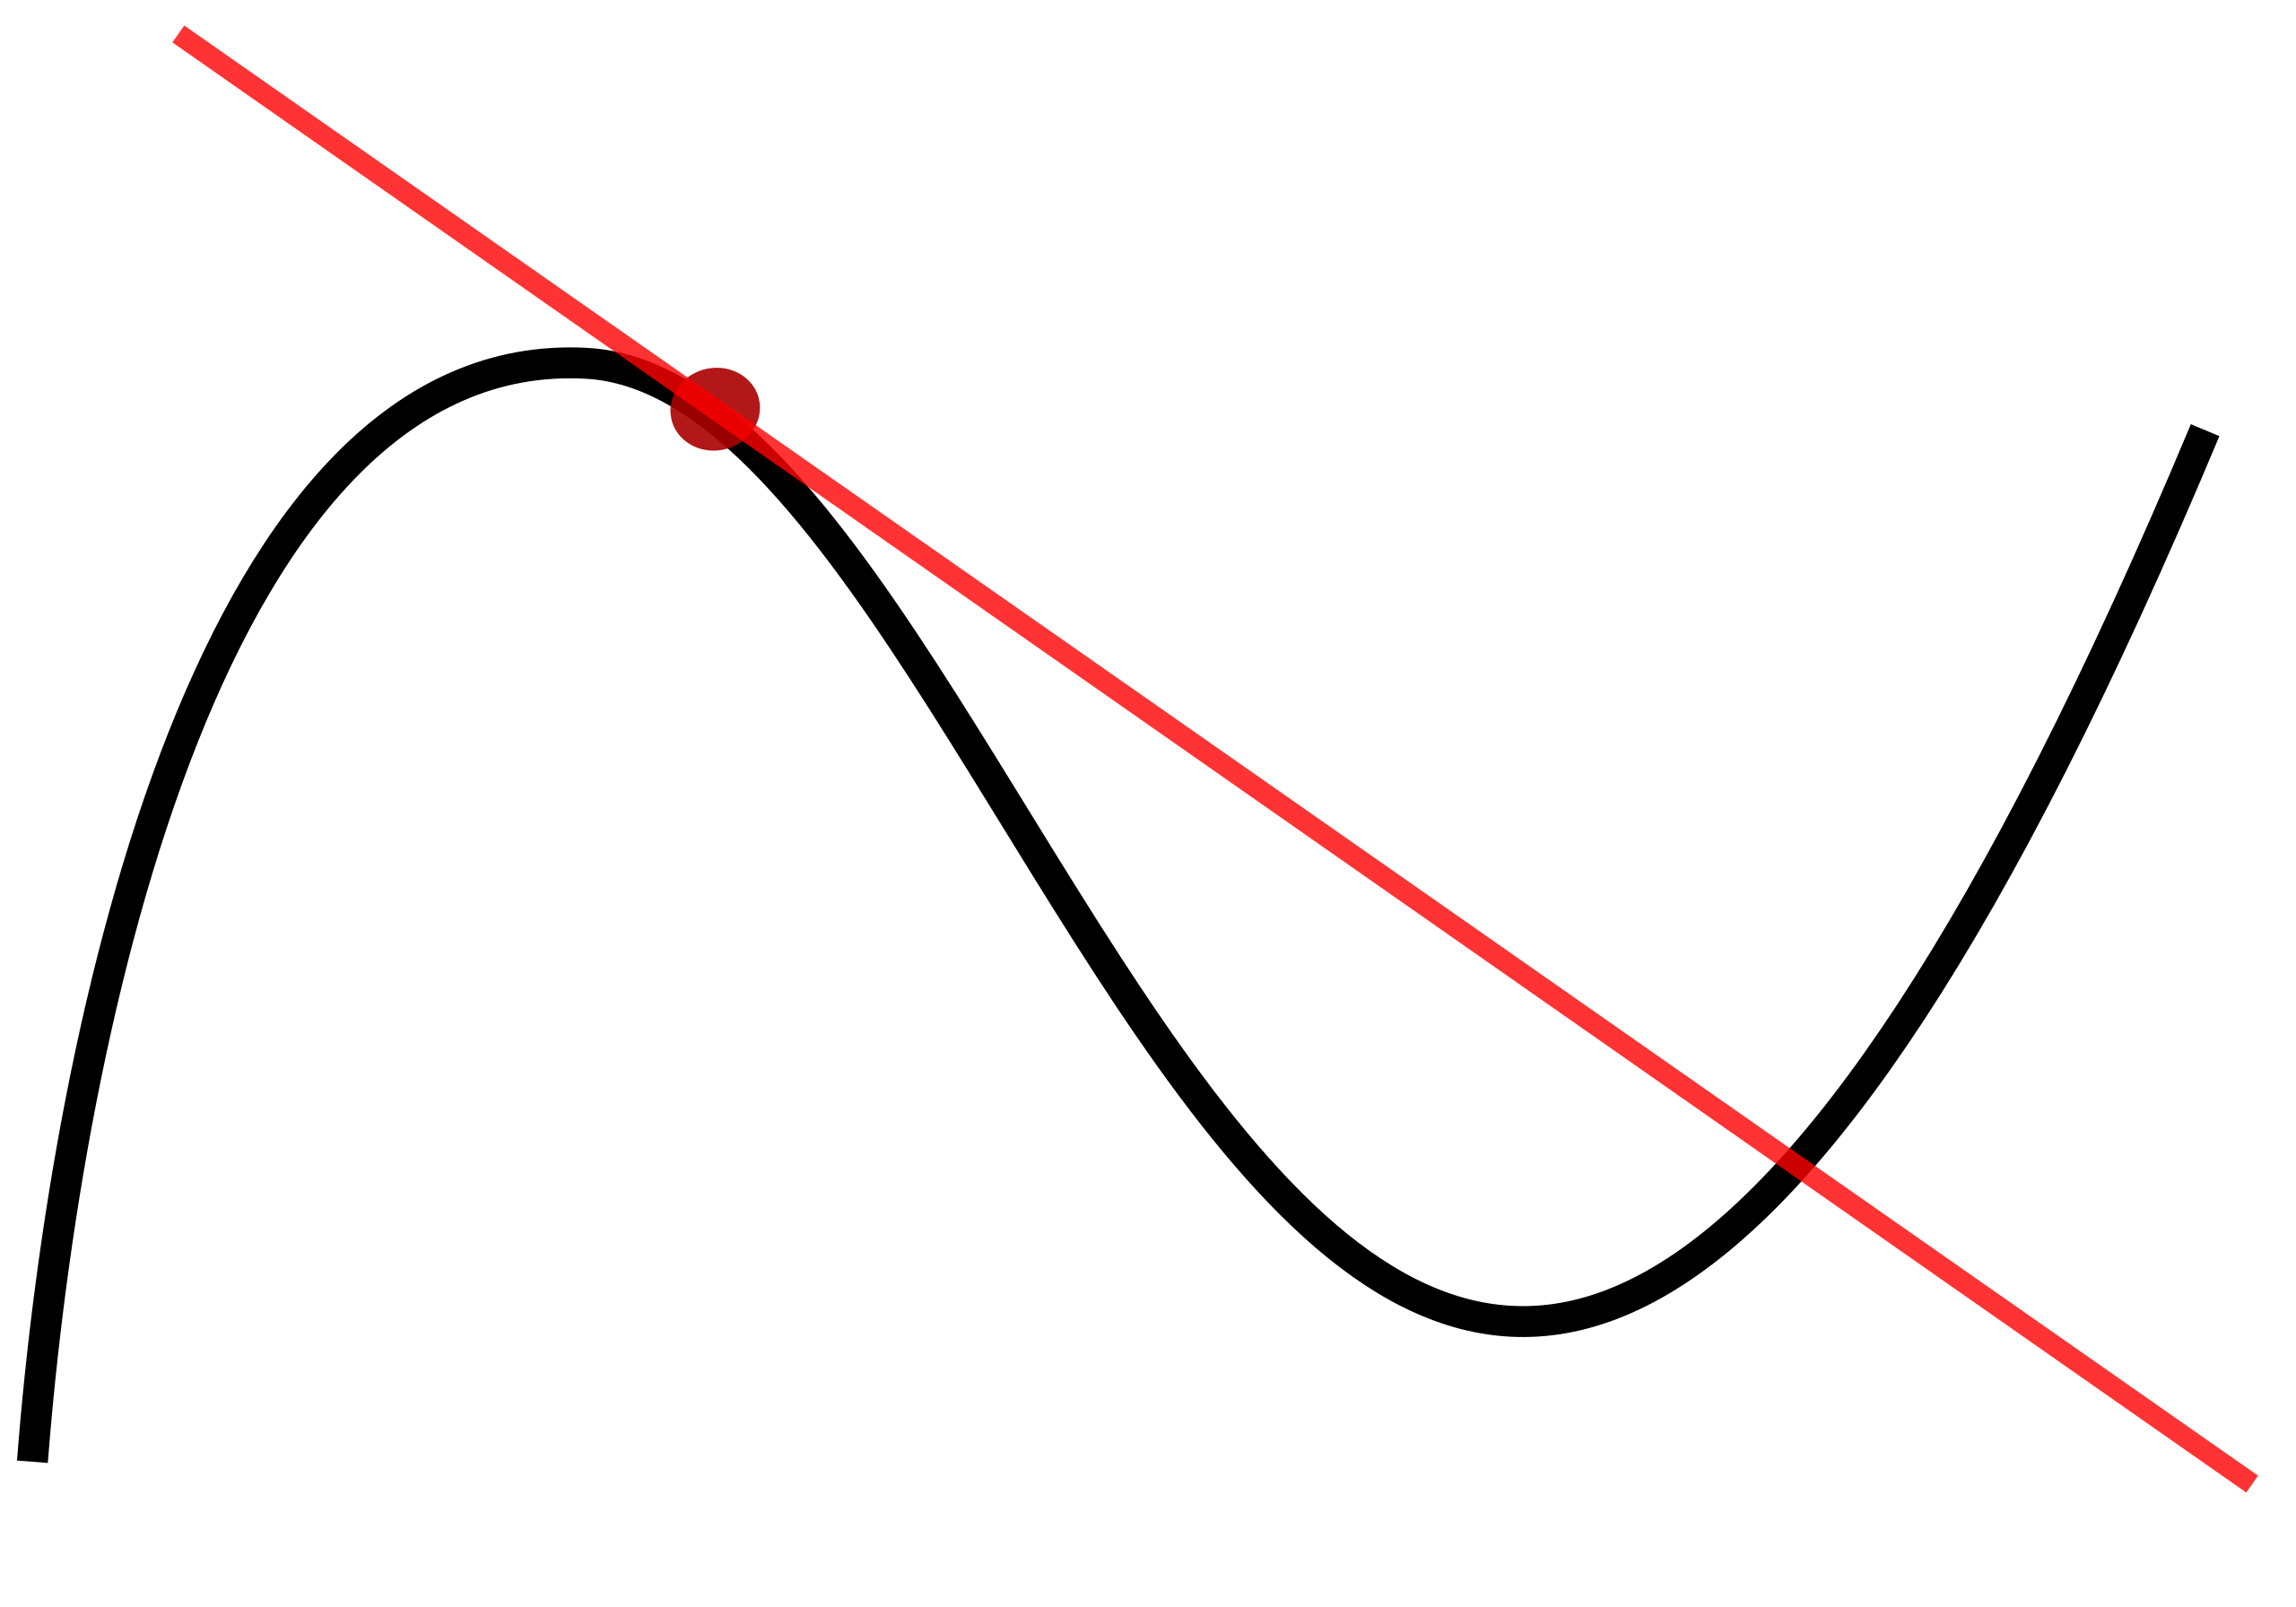
\includegraphics[width=0.3\textwidth, alt ={A schematic of the derivative as a tangent to a curve.}]{figures/Tangent_to_a_curve}
    %}{A schematic of a derivative as a tangent to a curve. }
    \caption{The derivative of a function at a point is equivalent to finding the tangent to a curve at this point.  }
\label{fig: derivative as tangent}
\end{figure}

\begin{figure}[ht]
    \centering
   % \pdftooltip{
   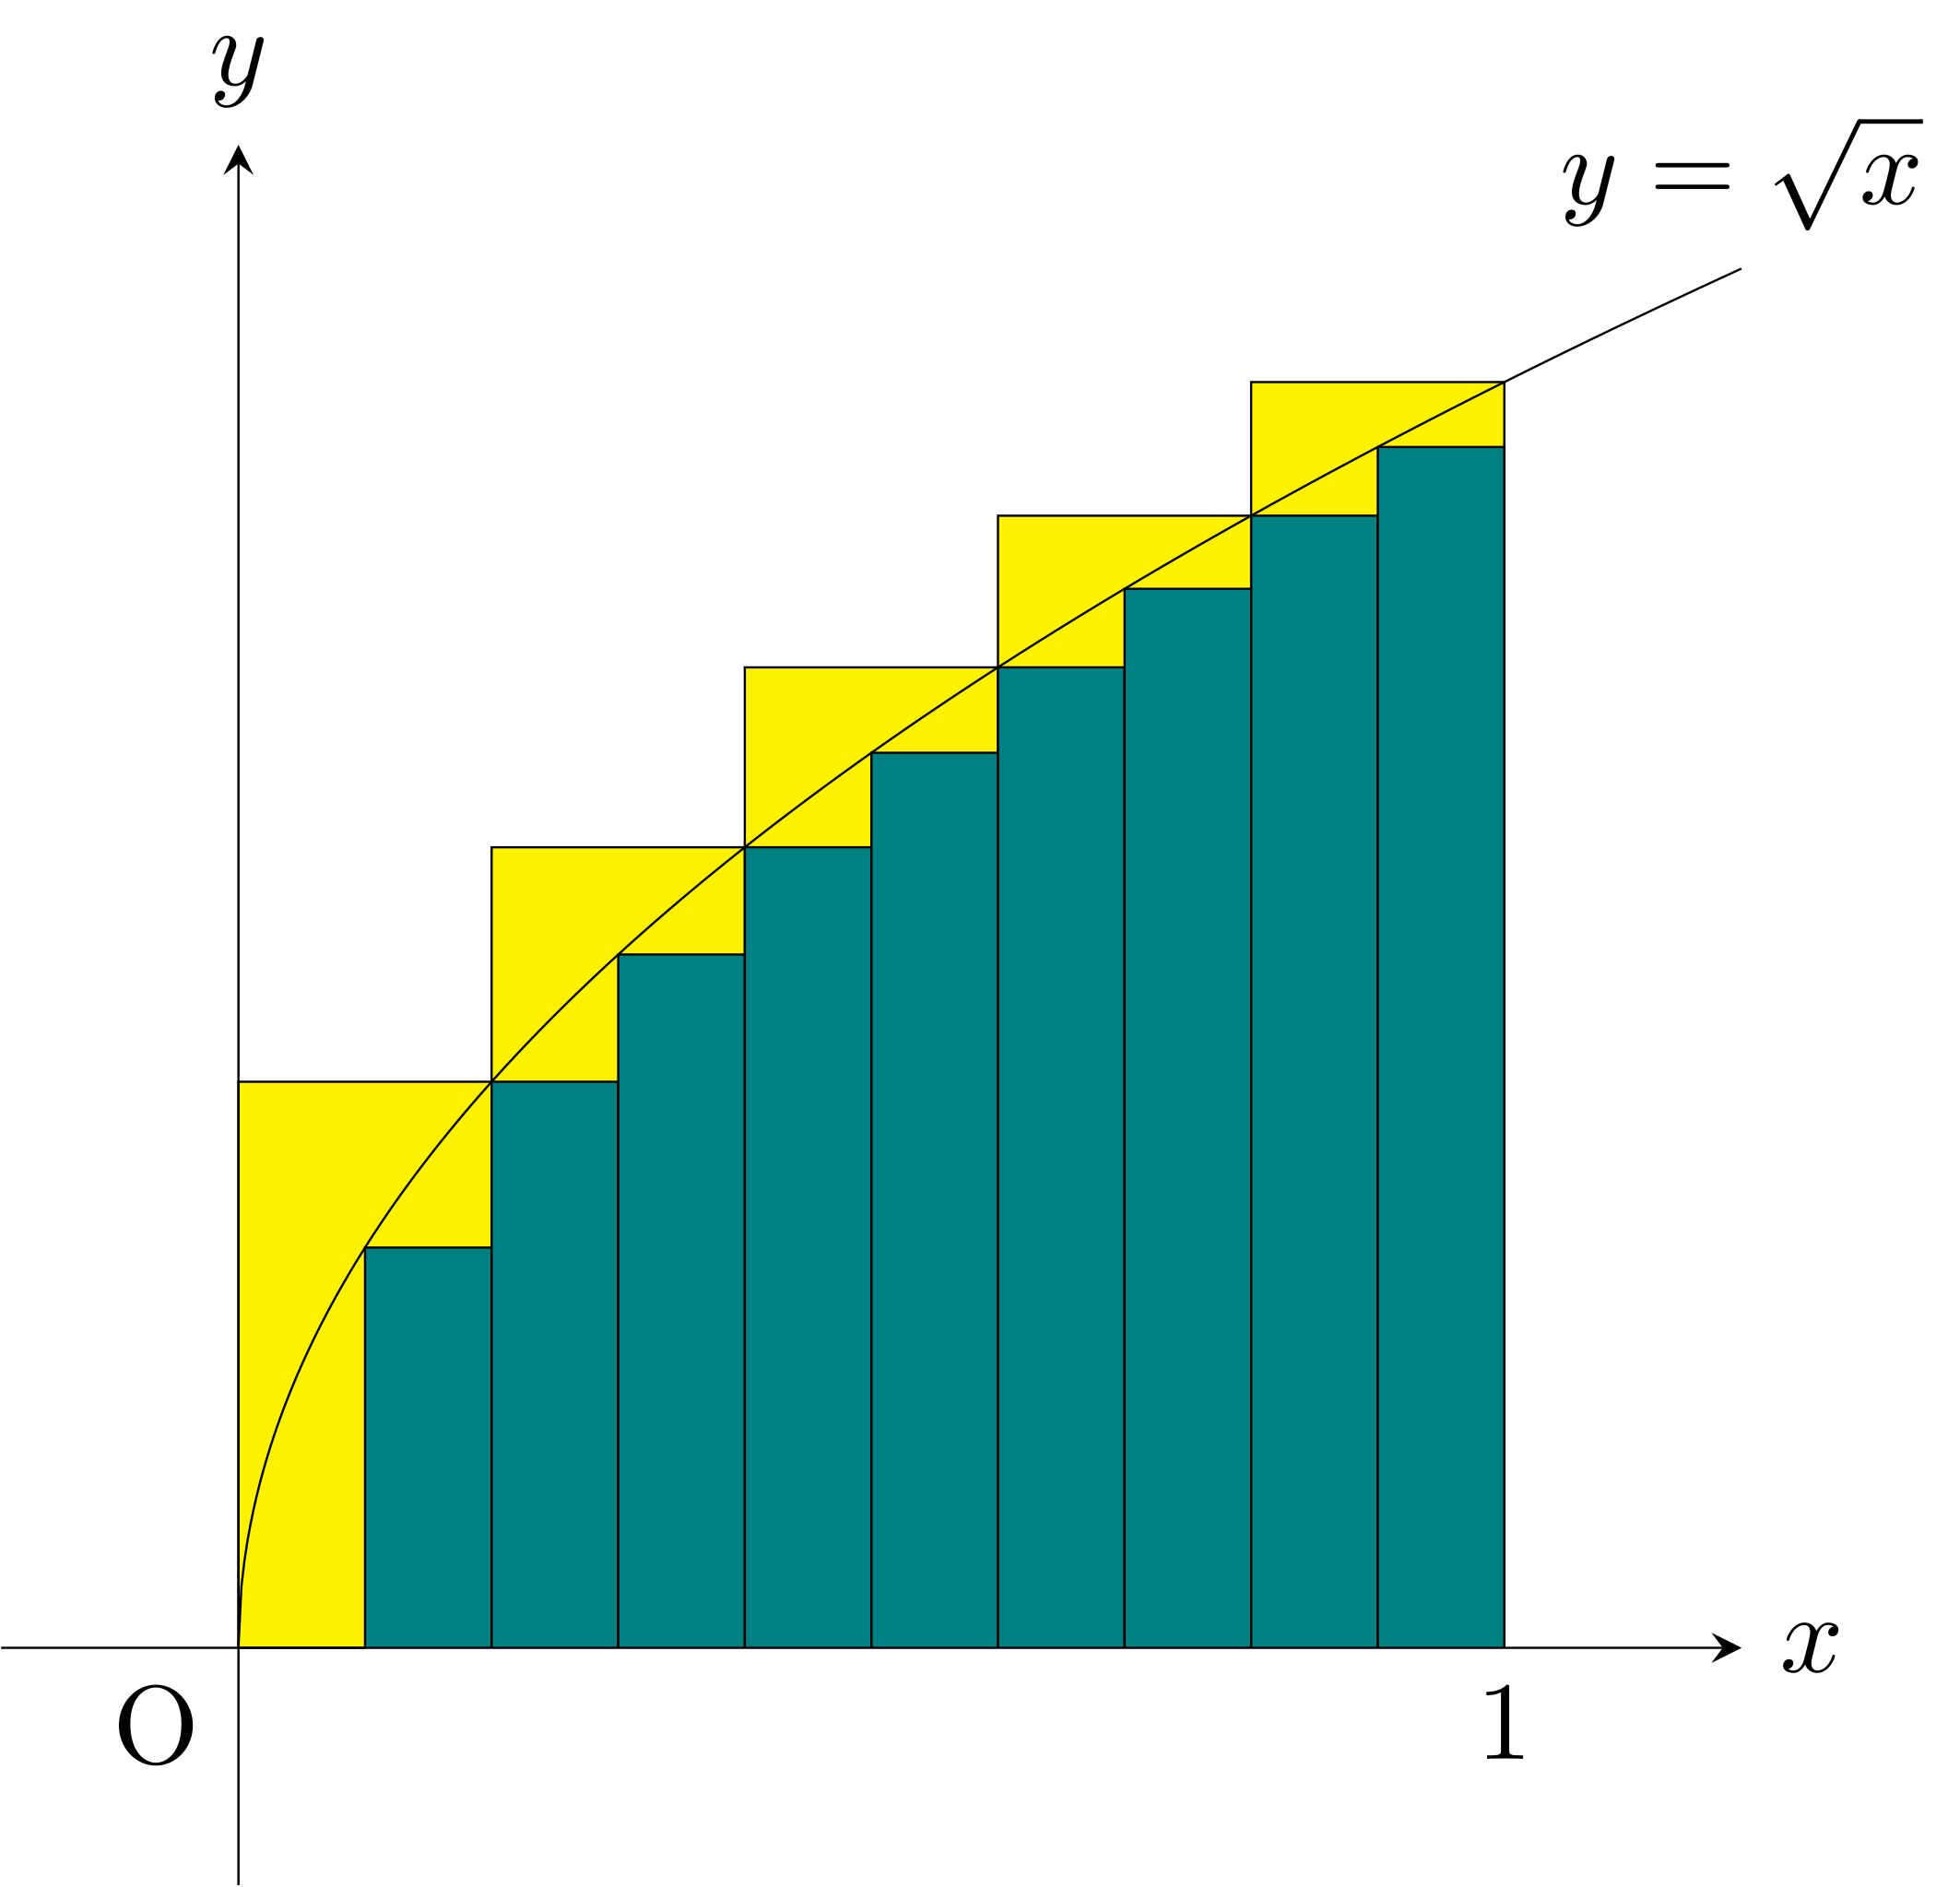
\includegraphics[width=0.4\textwidth, alt ={A schematic of an integral as the area under the curve.}]{figures/Integral_approximations}
   %}{A schematic of an integral as the area under the curve. }
    \caption{The integral, or area under the curve, can be approximated by rectangles. Depending on the size of the rectangles this can be an over estimate or an underestimate, but it will improve the thinner the rectangles become. This figure comes from \href{https://commons.wikimedia.org/wiki/File:Integral\_approximations\_J.svg}{Wikimedia Commons}. }
\label{fig: integral approximation}
\end{figure}
The YouTube channel 3Blue1Brown has an excellent playlist called the essence of calculus available \href{https://www.youtube.com/playlist?list=PLZHQObOWTQDMsr9K-rj53DwVRMYO3t5Yr}{here} which goes through the basics of calculus and its implications in a fairly unique way. Grant's goal in the videos is to give you an intuition for why Calculus works the way it does, rather than just giving you a list of facts and equations to memorise. Hopefully you will find that this module takes a similar approach, the goal is for you to understand the how and why of the mathematics and not just approach it as a set of rules to memorise. \\

If you find that you enjoy any of the topics in this module, or just want to read about interesting mathematics in a popular science setting I recommend having a look at \href{https://chalkdustmagazine.com/}{\textit{\gls{Chalkdust}} magazine}. As one of the editors of \textit{Chalkdust} I may be biased, but I think that it is a nice way to find out about some interesting maths without having to go into all of the details.\\

Hopefully, this has given you a feel for why you are doing this module. Now we can get started with the mathematics. As calculus is the study of how functions change we first need to remind ourselves of some of the properties of functions and introduce some notation.

\section*{How to use these notes }
As stated above, these notes are here to complement the in person lectures rather than to replace them.  For some topics there will be more detail given here, while at other points there may be explanations that I give in the lectures, or examples that I use which do not appear in these notes.  Also, I will frequently draw pictures in the lectures, as the module goes on I will try to add these figures to the lecture notes. However, that will not always be possible. These notes also contain exercises, some of which will appear in the tutorial sheets, that you should solve to help reinforce the concepts from the module.\\

To complement the theory presented in these notes you will find a range to examples and exercises to help you build familiarity with the mathematical concepts that we will meet during this module. As this is not a module for mathematicians we will not always completely precise and give all the details, but rather focus on the practical applications of the mathematics. Occasionally I will include a \textbf{\gls{Mathematical Diversion}} where I give some more of these details. If you are interested in the mathematics for its own sake then these will hopefully be interesting to you. If you are only interested in the mathematics that you need to pass this module, then feel free to skip these diversions.\\

\begin{warpprint} % For print only output ...
These lecture notes will continue to develop as the module goes on so make sure to check back frequently to see what has been added. There is also an online html version of these notes that you can check out as well. The html version should be accessible with alttext on the figures. If you have any difficulty viewing either these notes or the html version let me know.
\end{warpprint}

